\subsection{Datenbankdesign}
Bei Design der Datenbank stellten sich einige grundlegenden Fragen:

\begin{itemize}
	\item Wie werden die Schulstunden gespeichert?
	\item Wie werden die Supplierungen gespeichert?
\end{itemize}

\subsubsection{Gewählte Lösung}
Die Gruppe entschied sich für folgende Lösung:\\
\\
Es gibt Tabellen für:\\
\begin{itemize}
	\item Abteilungen
	\item Klassen
	\item Klassen
	\item Fächer
	\item Lehrer
	\item Uhrzeiten
\end{itemize}
\vspace{0.03cm}
\begin{itemize}
	\item Die Basis-Stunden
	\item Die Stunden
\end{itemize}
\vspace{0.03cm}
\begin{itemize}
	\item fehlende Lehrer
	\item fehlende Klassen
\end{itemize}
\vspace{0.03cm}
\begin{itemize}
	\item Die Supplierung
\end{itemize}
Die Basis-Stunde verknüpft die Klasse der Stunde mit der Uhrzeit. Die Stunde verknüpft die Basis-Stunde mit dem Lehrer, dem Fach und dem Raum.\\
\\
Die Basis-Stunde wird benötigt, damit die Information, welche Klasse wann Unterricht hat, nicht mehrfach gespeichert werden muss.\\
\\
Die Tabellen für die fehlenden Lehrer und die fehlenden Klassen haben Spalten für eine Start- und End-Zeit.\\
\\
Die Supplierungs-Tabelle hat Felder für die Stunde, den Supplierlehrer, den neuen Klassenraum, die neue Start- und Endstunde, sowie Flags zum Ausblenden der Stunde auf dem angepassten Stundenplan.\\
Es ist möglich, mehrere Supplierungen für die gleiche Stunde einzutragen. Dieses Verhalten ist für manche Ausnahmefälle notwenig (siehe Beispiel).\\
\\

\begin{figure}[H]
\centering
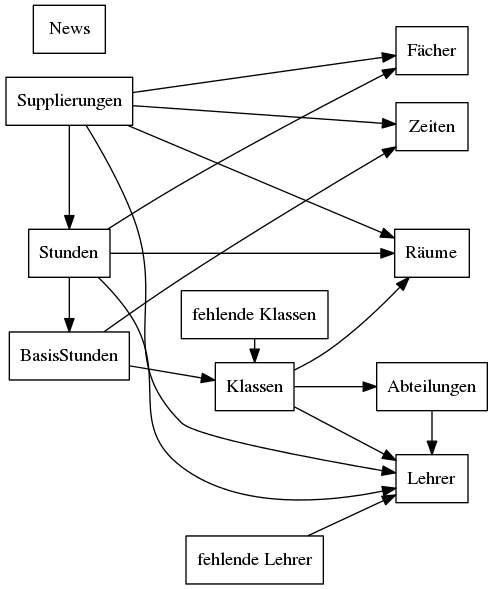
\includegraphics[keepaspectratio=true, width=10cm]{images/dbSubstitudes.png}
\caption{Supplierungs-Datenbank}
\end{figure}

Für das folgende Beispiel wird angenommen, dass eine Schulstunde 60 Minuten entspricht.\\
\textit{Beispiel:} Klasse K hat am Montag um 8:00 eine Doppelstunde des Faches F mit Lehrer L in Raum R. Da der Lehrer zu spät kommen wird (ist bereits im vorhinein bekannt), soll nun die erste Stunde auf 16:00 in Raum P verschoben werden, die zweite Stunde soll aber bleiben.\\
\textit{Lösung:} Die Doppel-Stunde wird 2 mal suppliert. Einmal mit dem selben Lehrer im selben Raum mit Start-Stunde um 9:00 und End-Stunde um 10:00. Und das zweitemal mit dem selben Lehrer im Raum P mit Start-Stunde um 16:00 und End-Stunde um 17:00.

\subsubsection{Alternative Lösungen}

Eine alternative Lösung, die angedacht wurde, ist folgende:\\
\\
Ansatt zwei Tabellen für die Basis-Stunde und die Stunde gibt es nur eine Stunden-Tabelle.
Diese verknüpft die Klasse mit der Uhrzeit, der Länge der Stunde, einem kombinierten Lehrer-Feld, einem kombinierten Fächer-Feld, einem kombinierten Raum-Feld.\\
\\
Die kombinierten Felden sollten den ersten Wert enthalten. Für jeden weiteren Wert wird der aktuelle Feld-Wert verodert mit dem nächsten Wert, welcher zuvor um ($x \cdot $(Anzahl der bisherigen Einträge)) Bits nach links verschoben wurde.\\
Hierbei wurde \textit{x} noch nicht bestimmt, es müsste so gewählt werden, dass der Eintrag mit der höchsten ID nicht in den dahinterliegenden Einträg überläuft (Für die Lehrer wäre $2^{8}$ (=256) ideal, da es knapp unter 200 Lehrer an der HTL gibt).\\
\\
Diese Lösungsmöglichkeit wurde allerdings verworfen, da es einiges an Aufwand ist, immer die richtigen Lehrer herauszulesen und da das Holen der Lehrer-Daten (Name, etc) nicht mehr im selben Query ausgeführt werden kann, als das Holen der Stundendaten, was bei mehr als 1 Zugriffspunkt zu Problemen mit der Daten-Konsistenz führen kann.